\documentclass[11pt]{article}
\usepackage{algorithm}
\usepackage{algorithmicx}
\usepackage{algpseudocode}
\usepackage{amssymb}
\usepackage{amsthm}
\usepackage{amsmath}
\usepackage{bm}
\usepackage{bbm}
\usepackage{cite}
\usepackage{color}
\usepackage[inline]{enumitem}
\usepackage[top=1.5in,bottom=1in,right=1in,left=1in]{geometry}
\usepackage{graphicx}
\usepackage{hyperref}
\usepackage{listings}
\usepackage{placeins}
\usepackage{siunitx}
\usepackage{subfig}
\usepackage{todonotes}
\usepackage{wrapfig}
\usepackage{authblk}
\usepackage{mathabx}
\usepackage[english]{babel}
\newtheorem{theorem}{Theorem}[section]
\newtheorem{corollary}{Corollary}[theorem]
\newtheorem{lemma}[theorem]{Lemma}


\title{Title}
\author[1]{Stefan Caldararu}
\affil[1]{Undergraduate Student with Department of Computer Science, UW-Madison}
\date{\today}                     %% if you don't need date to appear
\setcounter{Maxaffil}{0}
\renewcommand\Affilfont{\itshape\small}


\newcommand{\comment}[1]{{\color{red}\textbf{#1}}}
\newcommand{\CC}{C\nolinebreak\hspace{-.05em}\raisebox{.4ex}{\tiny\bf +}\nolinebreak\hspace{-.10em}\raisebox{.4ex}{\tiny\bf +} }
\newcommand{\KS}{$K$-Server }
\newcommand{\s}{$\sigma$ }

\theoremstyle{definition}
\newtheorem{definition}{Definition}[section]


% \title{An Analysis of K-Server algorithm performance}
% \author[1]{Stefan Caldararu}
% \author[2]{Marc Renault}
% \affil[1]{Undergraduate Student with Department of Computer Science, UW-Madison}
% \affil[2]{Professor in the Department of Computer Science, UW-Madison}
% \renewcommand\Affilfont{\itshape\small}

\begin{document}
\maketitle
% \begin{titlepage}
% 	\begin{center}
% 		University of Wisconsin-Madison \\
% 		\vfill 
% 		\maketitle
% 		\vspace{0.2in}
% 		{\normalsize Department of Computer Science, University of Wisconsin -- Madison}	
% 		\vfill		
% 		\today		
% 	\end{center}
% \end{titlepage}

% \newpage 
% \vspace{0.1in}
\begin{center}
	Department of Computer Science\\
	University of Wisconsin -- Madison, USA
\end{center}
\vspace{1.5in}
\begin{abstract} 
	In this work, we focus on the \KS problem, a well-known problem in the field of online algorithms. We provide an overview of various algorithms used to solve this problem, and provide a detailed analysis of the Work Function Algorithm~\cite{KS1990, OnlineComp1998}. We then transition to the Unifying Potential, a recently proposed method of analysis for the \KS problem~\cite{unifyingPotential2021}. We provide an overview of the definitions and proofs used in this method, and attempt to extend their methods to Reduced Caterpillar Graphs. Finally, we provide an open-source software framework for testing and comparing these algorithms, and provide some experimental results derived using this software.
\end{abstract}

{\textbf{Keywords}}: \KS, Online Algorithms, Bijective Analysis

\newpage 
% ADD PRELIMINARIES, LITERATURE REVIEW
\tableofcontents

\newpage

\section{Introduction}
\label{sec:intro}
\subsection{Outline}
\label{sec:out}
In this paper, we consider the \KS problem in a variety of contexts. First, we provide a description of the \KS problem, along with a literature review of historically relavent works. We end the introductory section demonstrating a proof of a lower bound for the problem, additionally introducing the infamous \KS conjecture~\cite{KS1988}. 

In section~\ref{sec:algos}, we provide a brief description of various algorithms that have been proposed and analyzed for the \KS problem. We provide a brief historical background on some of these algorithms, and formal definitions for how the algorithms run.

In section~\ref{sec:wfa}, we focus on the Work Function Algorithm, which has shown promise to be the algorithm that satisfies the \KS conjecture. We then provide and an in-depth proof of the $2k-1$-competitiveness of the Work Function Algorithm ($WFA$), and describe a reduction of the $WFA$ to an efficient implementation leveraging a Min-Cut Max-Flow computation.

Following this an in-depth literature review is provided of the Unifying Potential for the WFA~\cite{unifyingPotential2021}. Additionally, we provide some useful insights into a potential extension of this work for caterpillar graphs. 

Finally, we transition to an analysis of the algorithms described in section~\ref{sec:algos}, focusing on various other forms of analysis. We describe a \CC environment provided for practical testing of these algorithms. Finally, we provide some experimental analysis of the algorithms within the testing suite, extending the work done in~\cite{independantStudy2023}.

\subsection{Notations and Definitions}

We provide a few definitions of notation that will be used throughout the paper for clarity.

\begin{definition}
    A \textbf{request sequence} $\sigma = \{ r_1, r_2, ... r_n\}$ can be broken up into sub-parts, where for $i \leq n$, $\sigma_i = \{ r_1, r_2, ..., r_i\}$ represents the first $i$ requests from within the request sequence.
\end{definition}

\begin{definition}
    An algorithm is denoted by an abreviated name, with any generic algorithm being denoted as $ALG$.
\end{definition}

\begin{definition}
    An instance of the \KS problem consists of a metric space $M = (X,d)$, a number of servers $k >1$, an algorithm $ALG$, and a request sequence $\sigma = \{ r_1, r_2, ... r_n\}$. The \textbf{cost} inccured on this instance of the \KS problem is denoted as $ALG(\sigma)$.
\end{definition}

\begin{definition}
    A set $C$ of $k$ points from within the metric space $M$ that an algorithm $ALG$ is operating in is called a \textbf{configuration}, representing the locations of the servers. Additionally, the initial configuration before any requests have been processed is denoted $C_0$, and the configuration after $ALG$ has operated on the first $i$ requests is denoted $C_{i}$. Additionally, $C$ can be used to denote an arbitrary configuration after servicing some request sequence $\sigma_i$, in which case $C'$ denotes the configuration after servicing the next request, i.e. servicing the request sequence $\sigma_{i+1}$.
\end{definition}

\begin{definition}
    The distance between two configurations $A$ and $B$ can be computed as the minimum weight matching between the two sets, denoted $D(A, B)$.
\end{definition}

\subsection{Problem Description}
\label{sec:desc}
As described above, an instance of the \KS problem can be described by a metric space $M = (X, d)$, a number of servers $k>1$, and an input sequence $\sigma = (r_1, r_2, r_3, ..., r_n)$, where each $r_i$ corresponds to a point in the metric space. Each of the $k$ servers is assigned an initial starting location within the metric space (generally this is assumed to be the first $k$ requests of the input sequence). Following this, The sequence of requests is processed one at a time. When a request comes in, the given algorithm $ALG$ must decide on one of the servers to service the request. It must then move said server from it's current location $x$ to the request $r_i$. This incurs a cost of $c = d(x, r_i)$. The costs are then summed across the request sequence, giving the final cost incurred by the algorithm $ALG(\sigma)$. The goal is to have $ALG$ incur the smallest possible cost while servicing all of the requests in the sequence~\cite{OnlineComp1998}.
\\ \\
There are two major distinctions to be made between different classes of algorithms. The first is the classification of a "lazy" algorithm - one that only moves a server in order to service the current request. Non-lazy algorithms will process a request, and then potentially also move other servers preemptively in order to prepare for future requests. 

\begin{lemma}
    For any non-lazy algorithm $ALG$, there exists a lazy algorithm $LAZY$ such that $ALG(\sigma) \leq LAZY(\sigma)$.
\end{lemma}

\begin{proof}
    We can describe the algorithm $LAZY$ as follows: suppose we have our non-lazy algorithm, $ALG$. We have the algorithm $LAZY$ service requests with the same servers that $ALG$ services requests at each step. If $ALG$ were to move a server preemptively, $LAZY$ doesn't perform this move. Suppose that $ALG$ moves a server from location $x_1$ to location $x_2$ preemptively, and then later services request $r_i$ with this server. $LAZY$ will be servicing $r_i$ with the same server, except it will be moving directly from $x_1$ instead of $x_2$. By the triangle inequality, $d(x_1, r_i) \leq d(x_1, x_2) + d(x_2, r_i)$. By applying this principle throughout the request sequence, we will see that the cost of $LAZY$ will be as good if not better than that of $ALG$. By indexing the servers and ensuring that $LAZY$ services each request with the same server $ALG$ would, we have proven the lemma~\cite{OnlineComp1998}.
\end{proof}

The second major distinction is between "online" and "offline" algorithms. An offline algorithm receives the entire request sequence at once, and so as a result is able to make decisions on what server to use for the current request based off of future requests. In contrast, an online algorithm receives the request one at a time, and so is only able to make decisions based off of past requests, the current server configuration, and the current request. While online algorithms are at a severe disadvantage due to this, real world applications often rely on the performance of these algorithms. Applications range from disk access optimization, such as the two headed-disk problem~\cite{OnlineComp1998}, to police or firetruck servicing. In the context of this work, we will only consider an optimal offline algorithm $OPT$ as a comparison to the online algorithms we are analyzing.

\begin{definition}
    Any optimal offline algorithm is denoted as $OPT$.
\end{definition}

\subsection{Competitive Analysis}
\label{sec:compAna}
The most popular method for analyzing the performance of online algorithms for a problem is competitive analysis. Here, we assume a "malicious adversary", who is attempting to make our algorithm $ALG$ perform as poorly as possible in relation to the performance of the optimal algorithm $OPT$. The malicious adversary is allowed to come up with any finite input, and our competitive ratio is determined by this. If for any finite input, we are able to guaruntee that $ALG$ has a cost within a certain ratio $c$ of $OPT$ (allowing for a constant additive factor), then we say that our algorithm is $c$-competitive~\cite{OnlineComp1998}. So, then we have the following definition: 

\begin{definition}
\label{def:comp}
Algorithm $ALG$ is said to be \textbf{\textit{c}-competitive} if for every finite request sequence \s, $ALG(\sigma) \leq c\cdot OPT(\sigma)+\alpha$ for some constant $\alpha$.
\end{definition}

Competitive analysis is in some sense similar to "worst case" analysis, where we try to see how poorly an algorithm will ever perform. It is worth noting that some algorithms such as a greedy algorithm may perform very well on the majority of inputs, but given specific inputs may not be competitive at all. That is, given some value $c$, a finite length input can be found such that the algorithm doesn't satisfy the above definition~\cite{OnlineComp1998}.

\subsection{Literature Review}

The \KS problem originally arose as an abstraction of the paging problem, where the goal is to minimize the number of page faults in a cache as new memory access requests come in. It was originally proposed by Manasse, McGeoch, and Sleator~\cite{KS1988}, where they also showed a $2$-competitive 2 server algorithm for any metric space. They additionally demonstrated a $k$-competitive algorithm for metric spaces with $k+1$ points. Two years later they wrote a paper showing generally competitive algorithms and some applications~\cite{KS1990}. Manasse, McGeoch and Sleator additionally proposed the $k$ server conjecture: that is, that there exists a $k$-competitive algorithm for any metric space with $k$ servers. 

Following this, various algorithms were proposed with improving competitive ratios~\cite{KS1990, harm2000}. Koutsoupias and Papadimitriou~\cite{KS1990} showed that the Work Function Algorithm is $2k-1$-competitive in 1994, which to-date remains the best competitive ratio for the \KS problem for generic metric spaces.

Various other algorithms have been constructed for special metric spaces, most notably including the Double Coverage algorithm for line metric spaces~\cite{new1991}. This algorithm was later generalized to a $k$-competitive algorithm for trees~\cite{tree1991}.

The work function algorithm remains the strongest candidate for a $k$-competitive algorithm for the \KS problem. Various improvements have been made, including a proof that the work function algorithm is $k$-competitive on various classes of the problem. These include line metric spaces, metric spaces with $k+1$ points, metric spaces with $k+2$ points, multiray spaces (where there is a single "center" point, with rays extending out from it, i.e. only one node is connected to more than 2 other nodes), on tree graphs for $k=3$~\cite{unifyingPotential2021}, and on the Manhattan Plane for $k=3$~\cite{MP2002}. 

Most recently, in 2021 a paper by Coester and Koutsoupias proposes a new potential function for proving the competitiveness of the work function algorithm~\cite{unifyingPotential2021}. This paper proposes a \textit{unifying potential} that can be used to prove various subcases of $k$-competitiveness for the \KS problem. This shows promise as previous proofs relied on a variety of different potential functions, that were often non-generalizable to other cases.
%other forms of analysis / other results.
Additionally, other forms of analysis and modifications to the \KS problem have been proposed. Analysis methods include Direct Analysis where the cost of the algorithm is directly compared to the cost of the optimal algorithm on a given request sequence, and Max-Max ratios where the maximum cost of an algorithm on a set of inputs is compared to the maximum cost of another on the same set~\cite{MAXMAX2005}. Bijective Analysis and its generalization (Stochatic Dominance) have been proposed as methods for comparing algorithms. These methods favor algorithms that are able to consistently outperform other algorithms on a given set of inputs~\cite{bij2016}. 

Modifications to the \KS problem primarily include randomized algorithms, where the algorithm is allowed to make random decisions in order to improve its average case performance~\cite{OnlineComp1998}. Additional modifications include adding advice or lookahead for the algorithm. Great improvemenets can be made in an algorithms competitive ratio if it is able to get some sort of information, either about the current configuration of $OPT$, or about where the next few requests will be~\cite{advice2015}.

\subsection{$k$-competitive lower bound}
\label{sec:lowerBound}

In this section, we follow a proof for a lower bound of the $k$ server problem, as described in~\cite{server2009}.

\begin{lemma}
    For a metric space $M$ where $|M| > k$, no online algorithm $ALG$ can have competitive ratio less than $k$
\end{lemma}

\begin{proof}
    We begin by restricting all requests to a sub-metric space which has $k+1$ points. Within this metric space, there are $k+1$ possible configurations of the $k$ servers. We begin by maintaining $k$ offline algorithms (denoted $OPT_1, OPT_2, ..., OPT_k$), where each of these algorithms has a different configuration, and none have the same configuration as $ALG$. We denote the configuration of $ALG$ as $C = \{ x_1, x_2, ...x_k \} \in M$. We begin by requesting the point $r \not \in C$. All of the offline algorithms are able to service this request without moving any servers, while $ALG$ must move some server from $x_i$ to service this point. At this point we will have $OPT_i$, the offline algorithm that has no server at $x_i$, move its server from $r$ to $x_i$ preemptively. We then repeat this process.

    This shows that the cost incurred by $ALG$ will be equal to the sum of the costs incurred by all of the offline algorithms, showing that the competitive ratio of $ALG$ will be at least $k$.
\end{proof}

\section{Algorithms}
\label{sec:algos}

\subsection{Random Algorithm}
\label{sec:rand}
The random algorithm \textit{RAND} is the most basic of all of the online algorithms, and has little practical use. If the request is not currently covered by a server, then \textit{RAND} randomly selects one of it's servers, and moves the selected server to the service point. This algorithm is mostly just used as a baseline, as we would hope that none of the other algorithms will perform worse than random.

\subsection{Greedy Algorithm}
\label{sec:greedy}
The greedy algorithm \textit{GREEDY} is also a computationally inexpensive online algorithm, but which has many practical uses. This algorithm checks the distance that each server would have to travel to get to the service point, and selects the server which would incur the smallest cost. While this algorithm has very good performance for the majority of practical application inputs, it is surprisingly not a competitive algorithm~\cite{OnlineComp1998}. \textit{GREEDY} is one of the primary focuses of this study, as it is often looked over due to it's non-competitiveness, but still performs very well in practice.

\subsection{Optimal Algorithm}
\label{sec:OPT}
Any optimal offline algorithm \textit{OPT} is simply defined as an algorithm that will have the smallest possible cost for any request sequence. Computationally, the fastest implementations leverage a reduction to a Min Cost Max Flow problem. This reduction can be further studied in~\cite{WFA2009}. This still ends up being a good bit more computationally expensive than the previous algorithms, but is needed to be used as a metric to compare algorithms against, as most algorithms are compared to the optimal when determining their strenghts.

\subsection{Work-Function Algorithm}
\label{sec:WFA}
The Work-Function Algorithm \textit{WFA} is considered to be one of the most promising algorithms in terms of the competitive ratio, as it has been proven to be $(2k-1)$-competitive, and is believed to be $k$-competitive. Given a certain starting server configuration, current configuration, and previous input request sequence, \textit{WFA} determines which server an optimal algorithm would move, while also ensuring that $k-1$ of the servers end up in the current server configuration. This final server is then used to service the current request. A similar reduction to the \textit{OPT} computation can be used to find this server~\cite{WFA2009}. This means that the \textit{WFA} must compute a Min Cost Max Flow for each request, making it much more expensive than \textit{OPT}, and all of the other algorithms. Additionally, it is also worth noting that this is not a finite memory algorithm, as the WFA must remember all of the previous requests~\cite{MAXMAX2005}. 

\subsection{Double Coverage Algorithm}
\label{sec:DC}
The Double Coverage algorithm \textit{DC} is a $k$-competitive algorithm on the line. If the request is to the left of all of our current server locations, then we just move the left most server to service the request. If the server is to the right of all of the current locations, we use the rightmost server. Otherwise, the request will be between two servers. In this case, we move the two closest servers towards the reqeust at the same rate, until one of the servers reaches the request location. A proof of \textit{DC}'s competitiveness can be found in~\cite{OnlineComp1998}. It is also important to note that \textit{DC} is not a lazy algorithm, as it does move more than one server at a time. Additionally, generalizations of this algorithm can be used on metric spaces other than the line, such as trees.

\subsection{$k$-Centers Algorithm}
\label{sec:KC}
The $k$-Centers algorithm divides the metric space into $k$ sections, and assigns each server a section of the space to operate in. Implementations of this algorithm can either have the server return to the center of it's operating space after servicing the request in a non-lazy fashion, or just remember the bounds of each operating space, and service each request with the appropriate server~\cite{bij2016}.

\section{Work Function Algorithm}
\label{sec:wfa}
\subsection{Algorithm}
\label{sec:wfalg}
This section focuses on an in-depth analysis of the WFA. There are two ways of thinking about the WFA's decision-making process. WFA can be thought of as a balancing between retrospective-$OPT$, and a greedy algorithm. It tries to balance between the decisions $OPT$ would have made up until this point, assuming the current request is the last one that will be made, with a greedy algorithm that attempts to move the least distance possible at the current time step. This helps the algorithm maintain a configuration that is similar to $OPT$, without moving servers great distances from the current configuration.

Additionally, $WFA$ can be thought of from how it's implementation works. $WFA$ makes lazy decisions to move servers, so only moves one server at each step. As described previously, the $WFA$ will attempt to determine the server to move which would have the minimum cost for starting in an initial configuration, and ending with $k-1$ servers in the same locations they are currently in. Then, it will service the request with the server that does not stay in the initial configuration.

\subsection{Notations and Definitions}
\label{sec:notdef}

We begin with a couple of notation definitions for clarity.

\begin{definition}
    A set $C$ of k-points from within the metric space $M$ that an algorithm $ALG$ is operating in is called a \textbf{configuration}, representing the locations of the servers. Additionally, the initial configuration before any requests have been processed is denoted $C_0$, and the configuration after $ALG$ has operated on the first $i$ requests is denoted $C_{\sigma_i}$. Additionally, $C$ can be used to denote an arbitrary configuration after servicing some request sequence $\sigma_i$, in which case $C'$ denotes the configuration after servicing the next request, i.e. servicing the request sequence $\sigma_{i+1}$.
\end{definition}

\begin{definition}
    The distance between two configurations $A$ and $B$ can be computed as the minimum weight matching between the two sets, denoted $D(A, B)$.
\end{definition}

\begin{definition}
    The \textbf{work function}, denoted $w_\sigma(C)$ computes the minimum value required to begin in configuration $C_0$, service all requests in $\sigma$, and end with servers in configuration $C$. The work function has similar notation to configurations($w_{\sigma_i}$, $w$, and $w'$), except the work function value on an empty request sequence is denoted $w_\emptyset$. Additionally, the work function can be computed as follows:
    \begin{equation*}
        \begin{gathered}
            w_\emptyset(C) = D(C_0, C) \\
            w'(C) = min_{x \in C} \{ w(C - x + r) + d(x, r)\}
        \end{gathered}
    \end{equation*}
\end{definition}

\begin{definition}
    The \textbf{work function algorithm} moves the server currently at point $s$ at each step, incurring a cost $d(s,r)$. This server is determined as follows:
    \begin{equation*}
        s = argmin_{x \in C} \{ w(C-x+r) + d(x,r)\}
    \end{equation*}
\end{definition}
\subsection{$2k-1$ Proof}
\label{sec:2k1p}
In this section, we follow the proof showing that the $WFA$ is $2k-1$ competitive from~\cite{OnlineComp1998}, and add some in-depth explanatory details. 

It is worth noting a few basic property of the work function:

\begin{equation}
    \label{eq:nextwork}
    w'(C') = w(C') = w'(C) - d(s,r)
\end{equation}

\begin{equation}
    \label{eq:work}
    w'(C) = min_{x \in C} [w'(C - x + r) + d(r, x)] = min_{x \in C} [w(C - x + r) + d(r, x)]
\end{equation}

The first part of property~\ref{eq:nextwork} follows because $r \in C'$. The second part assumes that $s$ is the point from which the server that moved to service $r$, and follows from the definition of the WFA.

The first part of~\ref{eq:work} says that the work done to service a request sequence \textit{including} the next request $r$ for some configuration $C$ is equal to the minimum work done to service the same request sequence, except on the configuration $C$ without the point $x$ and with the point $r$, plus the distance between $r$ and $x$. The set $C-x+r$ is defined as in~\cite{OnlineComp1998}, where there is only one copy of $r$ in this set, whether or not $r$ was originally in $C$. 

The nice part about this is that we now \textit{know} that $r \in C - x + r$, which isn't necessarily true of $C$. This means that the second part of this equation is true, where we can remove the $r$ from the work function, as it is already included in the set. If $r \in C$, then the minimum is achieved by having $x = r$, because $d(r,x) = 0$ and therefore $w'(C) = w(C)$.

\begin{definition}
    The \textbf{offline pseudocost} $w'(C') - w(C)$ is the work done to service a request sequence $\sigma_{i+1}$ and end in configuration $C'$, minus the work done to service a request sequence $\sigma_i$ and end in configuration $C$.
\end{definition}

The offline pseudocost is a measure of how much work is done to service the next request in the sequence, given that the current configuration is $C$. If we sum this across all requests on sets $C_0$, $C_1$ ... $C_n$ for the configuration of \textit{OPT}, we will see that this will telescope to $w_{\sigma}(C_n) - w_{\emptyset}(C_0)$, where $\sigma_0 = \emptyset$. This is equal to the cost $OPT(\sigma)$, as we are subtracting the cost to get into the initial configuration $C_0$ from the final work function $w_\sigma(C_n)$.

\begin{definition}
    The \textbf{extended cost} is defined as $max_X \{ w'(X) - w(X)\}$.
\end{definition}

The extended cost represents the worst case configuration we could be in given the next request. That is, the configuration that will maximize the cost incurred to satisfy the next request. The extended cost represents the maximum cost we could incurr by servicing the next request online.

\begin{definition}
    A work function is \textbf{Quasi-Convex} (QC) if for all configurations $X$, $Y$, and for all $x \in X$, the following property holds:
    \begin{equation*}
        min_{y \in Y} \{ w(X - x + y) + w(Y - y + x)\} \leq w(X) + w(Y)
    \end{equation*}
\end{definition}

Quasi-Convexity essentially says that for every two configurations, the sum of the costs to get into those configurations is greater than or equal to the \textit{best} cost of swapping \textit{some} point $y\in Y$ with $x$. The key point here is that there will be some minimizing configurations $X$ and $Y$. We can additionally take this a step further with the following definition.

\begin{definition}
A work function is \textbf{General Quasi-Convex} (GQC) if for every $X$, $Y$, there exists a bijection $g: X \rightarrow Y$ such that for all partitions of X into $X_1$ and $X_2$, the following property holds:

\begin{equation*}
    w(X_1 + g(X_2)) + w(g(X_1) + X_2) \leq w(X_1) + w(X_2)
\end{equation*}
\end{definition}

It is worth noting that if a work function is GQC, then it is also QC. This is because we can set $X_1 = X-x$ and $y = g(x)$. This will give us the QC property.

\begin{lemma}
    If a bijection $g$ satisfies the GQC property, then there exists a bijection $\tilde{g}$ that satisfies the GQC property such that $\tilde{g}(x) = x$ for all $x \in X \cap Y$.
\end{lemma}
\begin{proof}
    Suppose we have a bijection $g: X \rightarrow Y$ that satisfies the GQC property, and additionally of all such bijections, maps the \textit{maximum} number of elements in $X \cap Y$ to themselves. by contradiction, assume that there exists some $a \in X \cap Y$ such that $g(a) \neq a$. Now, we define $\tilde{g}: X \rightarrow Y$ such that:
    
    \begin{equation*}
        \tilde{g}(x) = \begin{cases}
            g(x) & \text{if } x \neq a \text{ or } x \neq g^{-1}(a) \\
            a & \text{if } x = a \\
            g^{-1}(a) & \text{if } x = g^{-1}(a)
        \end{cases}
    \end{equation*}
    
    Now, let $(X_1, X_2)$ be a partition of $X$, and without loss of generality, $g^{-1}(a) \in X_1$. If $a \in X_1$, then $g(X_1) = \tilde{g}(X_1)$, and $g(X_2) = \tilde{g}(X_2)$, and so $\tilde{g}$ satisfies the GQC property, which is a contradiction to our second assumption. Therefore, $a \not\in X_1$, and so we have:

    \begin{equation*}
        w(X) + w(Y) \geq w((X_1+a) \cup g(X_2-a)) + w(g(x_1+a) \cup (X_2-a))
    \end{equation*}

    By the definition of GQC. Then, since $a\not \in X_2$ and $g^{-1}(a) \not \in X_2$, we know that $g(X_2-a) = \tilde{g}(X_2-a)$, by the definition of $\tilde{g}$. Additionally, $g(X_1+a) = \tilde{g}(X_1+a)$, since $a, g^{-1}(a) \in X_1$. Therefore, we have: 
    
    \begin{equation*}
        \begin{gathered}
            w((X_1+a) \cup g(X_2-a)) + w(g(x_1+a) \cup (X_2-a)) \\
            = w((X_1+a) \cup \tilde{g}(X_2-a)) + w(\tilde{g}(X_1+a) \cup (X_2-a)) \\ 
            = w(X_1 \cup \tilde{g}(X_2)) + w(\tilde{g}(X_1) \cup X_2)
        \end{gathered}
    \end{equation*}

    We achieve the last equality because $a \in X_1$ and $a \not\in X_2$, so $X_1 - a = X_1$ and $X_2 - a = X_2$. This would mean that $\tilde{g}$ satisfies the GQC property, which is again a contradiction. Therefore, there exists a bijection $\tilde{g}$ that satisfies the GQC property such that $\tilde{g}(x) = x$ for all $x \in X \cap Y$.
\end{proof}

\begin{lemma}
All work functions are GQC, and so are therefore also QC.
\end{lemma}

\begin{proof}
    We prove this by induction on the length of the request sequence. Our base case has $i = 0$, where $w_{\emptyset}(X) + w_{\emptyset}(Y) = D(C_0, X) + D(C_0, Y)$. We consider two minimum weight matchings, whose values are $D(C_0, X)$, and $D(C_0, Y)$. Each $c_j \in C_0$ is mapped by $M_X$ to some $x_j \in X$ and by $M_Y$ to some $y_j \in Y$. We show that the bijection $g(x_j) = y_j$ satisfies the GQC property. Because X and Y are minimum weight matchings, $w(X) + w(Y)$ is an upper bound of $D(X, Y)$. By the difinition of $g$, we maintain the indeces of our points when transitioning $X \rightarrow C_0 \rightarrow Y$. By a pointwise approach, we see that we satsify the GQC property with equality. We can think of this as doubling the number of servers at locations in $C_0$ and then matching them to the points in $X$ and $Y$. Each point in $X$ and $Y$ will appear exactly once on either side of the equation.

    For the induction step, we assume $w$ satisfies the GQC property, and we now have a new request $r$. We show that $w'$ satisfies GQC. We know that there exists some $x \in X$ such that $w'(X) = w(X-x+r) + d(x,r)$, and similarly there exists some $y \in Y$ such that $w'(Y) = w(Y-y+r) + d(y,r)$. We know there exists a bijection $g: (X-x+r) \rightarrow (Y-y+r)$ that satsfies the GQC property, where $g(r) = r$. We define $\tilde{g}: X \rightarrow Y$ as follows:

    \begin{equation*}
        \tilde{g}(z) = \begin{cases}
            g(z) & \text{if } z \neq r \\
            y & \text{if } z = r
        \end{cases}
    \end{equation*}

    From here, we will have $X_{xr} = X - x + r$ and $Y_{yr} = Y - y + r$ for easier notation. Without loss of generality, assume that $x \in X_1$ for some partition $X_1, X_2$ of $X$. We have:

    \begin{equation*}
        \begin{gathered}
            w'(X) + w'(Y) = w(X_{xr}) + w(Y_{yr}) + d(r, x) + d(r, y) \\
            = w( (X_1-x+r) \cup g(X_2)) + w(Y_{yr}) + d(r, x) + d(r, y) \\
            \geq w((X_1-x+r) \cup g(X_2)) + w(g(X_1-x+r) \cup (X_2)) + d{x, r} + d{r, y} \\
            = w(X_{xr} \cup \tilde{g}(X_2)) + w((\tilde{g}(X_1) -y + r) \cup X_2) + d(x, r) + d(r, y) \\
            \geq w'(X_1 \cup g'(X_2)) + w'(g'(X_1) \cup X_2) 
        \end{gathered}
    \end{equation*}
\end{proof}

\begin{definition}
    Let $w$ be the current work function and let $r$ be any point in our metric space. A configuration $A$ is called a \textbf{minimizer of $r$ with respect to $w$} if:
    \begin{equation*}
        A = argmin_{(X)} \{ w(X) - \Sigma_{x \in X} d(x,r)\}
    \end{equation*}
\end{definition}

\begin{lemma}
    \label{lem:min}
    Let $w$ be the current work function and let $r$ be the next request. If $A$ is a minimizer of $r$ with respect to $w$, then $A$ is also a minimizer of $r$ with respect to $w'$.
\end{lemma}

\begin{proof}
    We want to show that for every $B$, $w'(A) - \Sigma_{a \in A} d(a,r) \leq w'(B) - \Sigma_{b \in B} d(b,r)$. This is equivalent to showing the following, as per property~\ref{eq:work}:
    
    \begin{equation*}
        \begin{gathered}
            min_{a' \in A} \{ w(A - a' + r) + d(a', r) - \Sigma_{a \in A} d(a,r)\} \leq min_{b' \in B} \{ w(B - b' + r) + d(b', r) - \Sigma_{b \in B} d(b,r)\}
        \end{gathered}
    \end{equation*}

    Since $A$ is a minimizer of $r$ with respect to $w$:

    \begin{equation*}
        \begin{gathered}
            w(A) - \Sigma_{a \in A} d(a,r) \leq w(B-b' + a') - \Sigma_{b \in B - b' + a'} d(b, r) \\ \\
            w(A) - w(B-b' + a') - \Sigma_{a \in A} d(a,r) \leq -\Sigma_{b \in B} d(b, r) + d(b', r) - d(a', r) \\ \\
            -w(B - b' + a') + w(A) + d(a', r) - \Sigma_{a \in A} d(a,r) \leq -\Sigma_{b \in B} d(b,r) + d(b', r)
        \end{gathered}
    \end{equation*}

    Now, we apply the GQC Lemma, with $X = B -b' + r$, $Y = A$, $x = r$, and $y = a'$. This means that $min_{a' \in A} \{ w(B - b' + a') + w(A -a' + r)\} \leq w(B - b' + r) + w(A)$. We now sum the two sides of this with the previous inequality to get the following equation:

    \begin{equation*}
        \begin{gathered}
            min_{a' \in A} \{ w(B - b' + a') + w(A -a' + r) - w(B - b' + a') + w(A) + d(a', r) + \Sigma_{a \in A} d(a, r)\} \\
            \leq w(B - b' + r) + w(A) + d(b' ,r) - \Sigma_{b \in B} d(b, r)
        \end{gathered}
    \end{equation*}

    And after cancelations, we get that for all $b' \in B$:

    \begin{equation*}
        \begin{gathered}
            min_{a' \in A} \{ w(A - a' + r) + d(a', r) - \Sigma_{a \in A} d(a,r)\} \leq w(B - b' + r) + d(b', r) - \Sigma_{b \in B} d(b,r)
        \end{gathered}
    \end{equation*}

    Since this is true for all $b' \in B$, our property holds for the $b'$ that minimizes the right hand side, completing our proof.
\end{proof}

\begin{definition}
    We define the \textbf{extended cost} as the cost of the value achieved by the configuration which is able to maximize the difference between the next work function value and the current work function value:
    \begin{equation*}
        max_X \{ w'(X) - w(X)\}
    \end{equation*}
\end{definition}

\begin{definition}
    Additionally, we define a \textbf{maximizer with respect to $w$} as the configuration $A$ which achieves this extended cost value:
    \begin{equation*}
        A = argmax_X \{ w'(X) - w(X) \}
    \end{equation*}
\end{definition}

\begin{lemma}
    \label{lem:dual}
    Any minimizer with respect to $r$ is also a maximizer with respect to $w$.
\end{lemma}

\begin{proof}
    Suppose $A$ is a minimizer with respect to $r$. We want to show that for every $B$,

    \begin{equation*}
        \begin{gathered}
            w'(B) - w(B) \leq w'(A) - w(A) \\ \\
            w'(B) + w(A) \leq w'(A) + w(B)
        \end{gathered}
    \end{equation*}

    If $r \in B$, then this statement is true, as $w'(B) = w(B)$, and $w(A) \leq w'(A)$ by definition.

    By expanding the above desired equation using eq.~\ref{eq:work}, we get that we want to show:

    \begin{equation*}
        \begin{gathered}
            min_{b' \in B} \{ w(B - b' + r) + d(b', r) + w(A)\} \leq min_{a' \in A} \{ w(A - a' + r) + d(a', r) + w(B)\}
        \end{gathered}
    \end{equation*}

    This is equivalent to saying that for all $B$, $a' \in A$: 

    \begin{equation*}
        \begin{gathered}
            min_{b' \in B} \{ w(B - b' + r) + d(b', r) + w(A)\} \leq w(A - a' + r) + d(a', r) + w(B)
        \end{gathered}
    \end{equation*}

    To show this, we begin with the statement that $A$ is a minimizer. In particular, this means that:

    \begin{equation*}
        \begin{gathered}
            w(A) - \Sigma_{a \in A} d(a,r) \leq w(A -a' + b') - \Sigma_{a \in A - a' + b'} d(a,r) \\ \\
            w(A) - \Sigma_{a \in A} d(a,r) \leq w(A -a' + b') - \Sigma_{a \in A} d(a,r) + d(a', r) - d(b', r) \\ \\
            w(A) + d(b', r) - d(a', r) \leq w(A - a' + b')
        \end{gathered}
    \end{equation*}

    When we apply the QC property with $X = A - a' + r$, $Y = B$, $x = r$, and $y = b'$, and then substitute in for $w(A - a' + b')$, we get:

    \begin{equation*}
        \begin{gathered}
            min_{b' \in B} \{ w(A - a' + b') + w(B - b' + r)\} \leq w(A - a' + r) + w(B) \\ \\
            min_{b' \in B} \{ w(A) + d(b', r) - d(a', r) + w(B - b' + r)\}\leq w(A - a' + r) + w(B) \\ \\
            min_{b' \in B} \{ w(B - b' + r) + d(b', r) + w(A)\} \leq w(A - a' + r) + d(a', r) + w(B)
        \end{gathered}
    \end{equation*}
\end{proof}

\begin{definition}
    \label{eq:MIN}
    We now define the \textbf{value of a minimizer configuration}, for minimizer $A$ of $r$ with respect to $w$ as: 
    \begin{equation*}
        MIN_w(r) = w(A) - \Sigma_{a \in A} d(a, r)
    \end{equation*}
\end{definition}

We now fix any optimal algorithm $OPT$, and have $U = \{u_1, u_2, ... , u_k \}$ as the current configuration of $OPT$. We will now have the potential function: $\Phi ( U, w) = \Sigma_{u \in U} MIN_w(u)$. Additionally, suppose that for the next request $r$, $OPT$ services the request with server $u_j$. Then, the next configuration of $OPT$ is $U' = U - u_j + r$.

\begin{lemma}
    \label{lem:ep1}
    $\Phi ( U', w) - \Phi (U, w) \geq k * d(u_j, r)$
\end{lemma}

\begin{proof}
    Using the triangle inequality, we know that for all $a$, $d(a, r) \leq d(a, u_j) + d(u_j, r)$. Putting the value of a minimizer together with this, we get:

    \begin{equation*}
        \begin{gathered}
            MIN_w(r) = min_A \{ w(A) - \Sigma_{a \in A} d(a, r)\} \\
            \geq min_A \{ w(A) - \Sigma_{a \in A} [d(a, u_j) + d(u_j, r)]\} = MIN_w(u_j) - k*d(u_j, r) \\ \\
            \Phi ( U', w) - \Phi (U, w) = \Sigma_{u \in U'} MIN_w(u) - \Sigma_{u \in U} MIN_w(u) \\ = MIN_w(r) - MIN_w(u_j) \geq MIN_w(u_j) - k * d(u_j, r) - MIN_w(u_j) = -k*d(u_j, r)
        \end{gathered}
    \end{equation*}
\end{proof}

\begin{lemma}
    \label{lem:ep2}
    $\Phi(U', w') - \Phi(U', w) \geq max_X \{ w'(X) - w(X)\}$
\end{lemma}

\begin{proof}
    Let $A$ be a minimizer of $r$ with respect to $w$. Again, we know that $w'(X) \geq w(X)$ for all $X$, as any sequence of moves that would service $\sigma r$ and end in configuration $X$ would also service requests $\sigma$ and be able to end in $X$ with the same or lesser distance traveled. Therefore, for any point $p$, we have: 

    \begin{equation*}
        MIN_{w'}(p) = min_{X} \{w'(X) - \Sigma_{x \in X} d(p,X) \} \geq min_{X} \{w(X) - \Sigma_{x \in X} d(p,X)  \} = MIN_w(p)
    \end{equation*}

    This means that $MIN$ is also monotone incresing with respect to the request sequence. We have:

    \begin{equation*}
        \begin{gathered}
            \Phi(U', w') - \Phi(U', w) = \Sigma_{u \in U'} (MIN_{w'}(u) - MIN_w(u)) \\
            = MIN_{w'} (r) - MIN_w(r) + \Sigma_{u \in U' - r} (MIN_{w'} (u) - MIN_w(u))\\
            \geq MIN_{w'} (r) - MIN_w(r)
        \end{gathered}
    \end{equation*}

    Because $A$ is a minimizer of $r$ with respect to $w$, we know by Lemma~\ref{lem:min} $A$ is also a minimizer of $r$ with respect to $w'$. So by using the duality lemma~\ref{lem:dual}, we have:

    \begin{equation*}
        \begin{gathered}
            \Phi(U', w') - \Phi(U', w) \geq MIN_{w'} (r) - MIN_w(r) \\
            = w'(A) - \Sigma_{a \in A} d(a,r) - [w(A) - \Sigma_{a \in A} d(a,r)]
            = w'(A) - w(A) = max_X \{ w'(X) - w(X)\}
        \end{gathered}
    \end{equation*}
\end{proof}

\begin{lemma}
    \label{lem:er1}
    $\Phi(U_\sigma, w_\sigma) \leq K * OPT(\sigma)$
\end{lemma}

\begin{proof}
     By the definition of $MIN$, we have:
     \begin{equation*}
        MIN_{w_\sigma}(u) = \leq min_{y \not \in U_\sigma} \{ w_\sigma(U - u + y) - \Sigma_{x \in U - u + y} d(x, u)\}
     \end{equation*}

     As the configuration $U$ with $u \in U$ minimizes the terms inside of the minimization on the right hand side. Suppose $y^*$ is a valid $y$ that minimizes the right hand side of the above equation. We have:
     
     \begin{equation*}
        \begin{gathered}
            MIN_{w_\sigma}(u) \leq w_\sigma(U - u + y^*) - \Sigma_{x \in U - u + y^*} d(x, u) \\
        \leq w_\sigma(U - u + y^*) - d(y^*, u) \leq w_\sigma(U_\sigma) = OPT(\sigma)
        \end{gathered}
     \end{equation*}

     When we sum over all $u \in U_\sigma$, we complete the lemma by the definition of $\Phi$
     
     \begin{equation*}
        \Phi(U_\sigma, w_\sigma) = \Sigma_{i=1}^k MIN_{w_\sigma}(u_i) \leq K * OPT(\sigma)
     \end{equation*}
\end{proof}

\begin{lemma}
    \label{lem:er2}
    For some constant $\alpha$ independent of $k$,
    \begin{equation*}
        \Phi(U_\emptyset, w_\emptyset) \geq - \Sigma_{a, b \in C_0} d(a, b) = \alpha
    \end{equation*}
\end{lemma}

\begin{proof}
    The sum in the middle of the above equation is clearly a constant that only depends on the initial configuration, and so therefore depends on the metric space, not directly on the number of servers. By definitions of $\Phi$ and $MIN$, we have:

    \begin{equation*}
        \Phi(U_\emptyset, w_\emptyset) = \Sigma_{u \in U_\emptyset} MIN_{w_\emptyset}(u) = \Sigma_{u \in U_\emptyset} min_X \{ w_\emptyset(X) - \Sigma_{x \in X} d(x, u)\}
    \end{equation*}

    Suppose $X^*$ is the configuration of servers which minimizes the right hand side for some $MIN_{w_\emptyset}(u) = min_X \{ w_\emptyset(X) - \Sigma_{x \in X} d(x, u)\}$. Without loss of generality, assume that $u_i$ matches to $x_i$ in the minimum weight matching between the two sets. Then, $w_\emptyset(X^*) = D(U_\emptyset, X^*)$. By using the triangle inequality, we get:

    \begin{equation*}
        \begin{gathered}
            MIN_{w_\emptyset}(u) = \Sigma_{i=1}^k d(u_i, x_i) - \Sigma_{i=1}^k d(x_i , u) \\
            = \Sigma_{i=1}^k [d(u_i, x_i) - d(x_i, u)] \geq \Sigma_{i=1}^k [d(u_i, x_i) - (d(u_i, x_i) + d(u_i, u))] = - \Sigma_{i=1}^k d(u_i, u) \\ \\
            \Sigma_{u \in U_\emptyset} MIN_{w_\emptyset(u)} \geq -\Sigma_{u \in U_\emptyset} \Sigma_{i=1}^k d(u_i, u) \\
            = - \Sigma_{a, b \in C_0} d(a, b)
        \end{gathered}
    \end{equation*}
\end{proof}

\begin{definition}
    We define the \textbf{total extended cost} as the sum over all moves of the extended costs.
    \begin{equation*}
        TEC = \Sigma_{i = 0}^{n-1} max_X \{ w_{i+1} (X) - w_i(X)\}
    \end{equation*}
\end{definition}

\begin{lemma}
    If the following property holds for some constant $\alpha$ independent of $\sigma$, then WFA is $c$-competitive:
    \begin{equation*}
        TEC \leq (c+1) * OPT(\sigma) + \alpha
    \end{equation*}
\end{lemma}

The above lemma follows directly by the provided definitions, because the total extended cost bouds the cost incurred by the work function algorithm. This lemma means that we are now only required to show the following:

\begin{lemma}
    $TEC \leq 2k * OPT(\sigma) + \alpha$, and therefore the $WFA$ is $2k-1$ competitive.
\end{lemma}

\begin{proof}
    By putting together lemmas~\ref{lem:ep1} and~\ref{lem:ep2}, we get:

    \begin{equation*}
        \Phi(U', w') - \Phi(U, w) \geq max_X\{ w'(X) - w(X)\} -k * d(u_j, r)
    \end{equation*}

    When we sum across all requests in the request sequence, we get the telescoping sum:

    \begin{equation*}
        \Phi(U_\sigma, w_\sigma) - \Phi(U_\emptyset, w_\emptyset) \geq TEC - k*OPT(\sigma)
    \end{equation*}

    By using lemmas~\ref{lem:er1} and~\ref{lem:er2}, we get:

    \begin{equation*}
        \begin{gathered}
            k * OPT(\sigma)+ \Sigma_{a, b \in C_0} d(a, b) \geq \Phi(U_\sigma, w_\sigma) + \Sigma_{a, b \in C_0} d(a, b) \\
            \geq \Phi(U_\sigma, w_\sigma) - \Phi(U_\emptyset, w_\emptyset) \geq TEC - k*OPT(\sigma)\\ \\
            TEC \leq 2k * OPT(\sigma) + \Sigma_{a, b \in C_0} d(a, b) = 2k * OPT(\sigma) + \alpha
        \end{gathered}
    \end{equation*}
\end{proof}
\subsection{Min-Cut Max-Flow Computation}
\label{sec:mcmf}
In this section, we describe a non-recursive implementation utilizing a min-cut max-flow formulation for the work function. 

\section{Unifying Potential}
\label{sec:uniPot}
In this section, we describe a unifying potential~\cite{unifyingPotential2021} that is a promising candidate for proving that the $WFA$ is $k$ competitive. Once again, we describe definitions and theorems taken directly from~\cite{unifyingPotential2021}. In section~\ref{sec:usefulInsights}, we provide some explanatory details of a few of the lemmas from the original paper, along with the proofs taken from the original work. In seciton~\ref{sec:cat}, we attempt to extend the work done in the original paper to a highly confined metric space - the reduced caterpillar graph.

The unifying potential is used to show that various subcases (ex. $k=2$, $k=n-1$, $k=n-2$, and various specialized metric spaces) are $k$ competitive. While many of these subcases have been shown to be $k$ competitive in the past~\cite{server1991, server2009, server1996, server2004, server2002}, the novelty of this approach is a \textit{single} potential function that is able to prove all of these cases. The authors of this unifying potential work take this as indication that it may be possible to prove the general $k$ competitiveness for the $WFA$ using this potential function.

\begin{definition}
    We define the notation $x^i$ to represent $i$ copies of the point $x$. That is, $w(x^k)$ represents the work done ending in the configuration where all $k$ servers are at the point $x$.
\end{definition}

\begin{definition}
    The \textbf{diameter} $\Delta$ of a metric space $M$ is defined as the largest distance between any two points in the metric space.
    \begin{equation*}
        \Delta = max_{x, y \in M} \{ d(x,y)\}
    \end{equation*}
\end{definition}

\begin{definition}
    A point $\bar{x} \in M$ is called an \textbf{antipode} of another point $x \in M$ if for every $y \in M$, $d(x,y) + d(y, \bar{x}) = \Delta$.
\end{definition}

It is worth noting that every metric space can be easily extended such that every point has an antipode. This is done by defining a copy of the original metric space, $\bar{M}$, where for every point $x \in M$, we have a copy $\bar{x} \in \bar{M}$. We denote the diameter of the original metric space $\Delta$. Distances within $\bar{M}$ and between the two spaces are defined as follows:

\begin{equation*}
    \begin{gathered}
        d(\bar{x}, \bar{y}) = d(x,y)\\ \\
        d(\bar{x}, y) = 2\Delta - d(x,y)
    \end{gathered}
\end{equation*}

The diameter of this extended metric space will be $2\Delta$, and every point will have an antipode. On an extended metric space $M \cup \bar{M}$ where every point $p \in M$ has an antipode $\bar{p} \in \bar{M}$, for any point $q \in M$ and any point $\bar{r} \in \bar{M}$, $d(p,q) \leq d(p,\bar{r})$. This just states that the cost for traversing to a node on the current subgraph you are on is \textit{always} less than or equal to the cost of traversing to the other subgraph.

\begin{definition}
    For a metric space $M$ where every point $x \in M$ has an antipode $\bar{x}$, we define the function \textbf{$\Phi_{x_1, x_2, ..., x_k}$} for a given configuration $x_1, x_2, ..., x_k$ as:

    \begin{equation*}
        \Phi_{x_1, x_2, ..x_k}(w) := \Sigma_{i=0}^k w(\bar{x_i}^i, x_{i+1}, ..., x_k)
    \end{equation*}
\end{definition}

\begin{definition}
    We define the \textbf{potential} $\Phi (w)$ as:

    \begin{equation*}
        \Phi(w) := min_{x_1, x_2, ..., x_k \in M} \Phi_{x_1, x_2..., x_k} (w)
    \end{equation*}
\end{definition}

\begin{lemma}
    For a metric space $M$ where every point has an antipode, If for every request $r \in M$ and for every work function $w_0$, $w_1$, ..., $w_n$ it holds that $\Phi(w) = \Phi_{x_1, x_2, ..., x_k}(w)$ for some $x_1, x_2, ...x_k \in M$ where $x_k = r$, then the $WFA$ is $k$ competitive on the metric space $M$.
\end{lemma}

While a proof for this is not provided here, we reference~\cite{unifyingPotential2021}, where a complete proof of this lemma is provided. This involves definition of a $n-k$ evader potential $\bar{\Phi}$, which is the dual to this problem. In this formulation, you have $n-k$ evaders in a metric space that must move away from requested points rather than towards them. It is clear that a solution to the evader problem would yield a parallel $k$ server solution.

\section{Experimental Analysis}
\label{sec:bijAna}

\subsection{Analysis Methods}
\label{sec:bijAnalysisDesc}
In this section, we present a few additional methods for analysis on algorithms other than competitive analysis. These methods are useful for comparing algorithms to each other, and can be used to demonstrate an algorithms efficiency outside of the "worst-case" considered by competitive analysis. Competitive analysis considers all requests of finite length. For each of these methods described below, we take an experimental-based approach. That is, each analysis method will be considerind the performance of an algorithm on a given request sequence length, and so can therefore be directly calculated in practice.

\subsubsection*{Direct Analysis}
\label{sec:Direct}
Direct analysis is a similar techinque to competitive analysis, in that we directly compare the performance of \textit{ALG} to the performance of \textit{OPT} on a request. Rather than looking across all request sequences of any finite length, we determine a specified length for our request sequence. Then, we look directly at the ratio of \textit{ALG}'s to \textit{OPT}'s performance for each input, and take the largest such ratio. It is important to note that as the length of our input approaches infinity, our direct analysis ratio will aproach the competitive ratio of our algorithm.

\begin{definition}
    \label{def:direct}
    Algorithm \textit{ALG} has a direct analysis ratio of $c$ if for every input \s of length $n$, $ALG(\sigma) \leq c\cdot OPT(\sigma)$.
\end{definition}

\subsubsection*{Max/Max Ratio}
\label{sec:MaxMax}
For the Max/Max ratio, we are comparing the worst case of each algorithm to each other. In practice, this makes sense to do on finite sets of input sequences. Here, we will take the highest cost of \textit{ALG} and the highest cost of \textit{OPT}, and this ratio will be our performance metric~\cite{MAXMAX2005}. 

\subsubsection*{Bijective Analysis}
\label{sec:Bij}
The bijective ratio is similar to using direct analysis, except we allow for a bijection between the two data sets. So, we look at the input space of all inputs of length $n$, denoted $I_n$. If there exists a bijetion $\pi:I_n \rightarrow I_n$ such that $ALG(\sigma) \leq c\cdot OPT(\pi(\sigma))$, then  we say that the bijective ratio between \textit{ALG} and \textit{OPT} is $c$~\cite{bij2016}. Therefore, we obtain def.~\ref{def:bij}. 

\begin{definition}
    \label{def:bij}
    For a given input space $I_n$, we say that algorithm \textit{A} has bijective ratio $c$ with respect to algorithm \textit{B} if there exists a bijection $\pi:I_n \rightarrow I_n$ such that $A(\sigma) \leq c\cdot B(\pi(\sigma))$, $\forall \sigma \in I_n$. 
\end{definition}

It is important to note that this definition doesn't only compare the ratio of an algorithm to the optimal, but can also be used to compare between two different online algorithms. This can be used to prove an online algorithms optimality~\cite{bij2016}, and allows for some interesting test-case results found in sec.~\ref{sec:analysis}.

\subsubsection*{Average Case Analysis}
\label{sec:Avg}
The average case analysis compares the average cost of two algorithms across a set of request sequences to each other. This is useful for comparing algorithms in practice, and additionally allows us to compare two algorithsm without storing their output for every input, which helps with both memory usage and storage usage.

\begin{definition}
    \label{def:avg}
    For a given input space $I_n$, we say that algorithm \textit{A} has an average case ratio $c$ with respect to algorithm \textit{B} if the average cost of \textit{A} is at most $c$ times the average cost of \textit{B} over all inputs of length $n$.
\end{definition}

\subsection{\CC Implementations}
\label{sec:implementation}
In this section, we describe the software package developed as part of this work. The package is written in C++, and has various levels of performance capabilities. It can additionally be run using the Lemon Graph Library~\cite{lemon}, or with purely internal data structure implementations. The various implementaiotns allow users to run the various algorithms described in sec.~\ref{sec:algos} either with a single thread, or under a producer-consumer framework for parallel processing. Additionally, a finite memory implementation is provided, and a memoization approach on the input sequence is implemented allowing for increased efficiency. Finally, example code for running the software on a High Throughput Cluster using Condor~\cite{htcondor} is provided.

\subsubsection*{Basic structures}

The most basic structure in the software package is the \texttt{Mspace} class. This class uses a \texttt{std::vector} to store the graph as an adjacency matrix of distances between nodes. Functions such as \texttt{setSize}, \texttt{getSize}, \texttt{getDistance}, and \texttt{setDistance} allow for easy manipulation of the metric space.

\texttt{getInput} and \texttt{writeOutput} classes are written to help maintain RAII standards, and allow for easy reading and writing of input and output files. 

An abstract \texttt{Alg} class is provided as a framework for each of the various algorithms to build off of. This class defines all basic functionality for an algorithm to run, and has a virtual function \texttt{run} that must be implemented by each algorithm, which takes an input request sequence and returns the cost incurred by the algorithm. It contains a \texttt{Mspace} object, and stores the current configuration of the servers in two forms: a \texttt{config} vector which stores the integer location of each server, as well as a \texttt{coverage} vector that stores whether or not each location in the metric space is covered by a server. This allows for efficient checking of whether or not a location is covered by a server, as well as efficient access to where the servers are located. \texttt{setServers} and \texttt{setGraph} functions are provided to allow for easy initialization of the algorithm, and a \texttt{moveServer} function is provided for easy manipulation of the server configuration.

\subsubsection*{Algorithm Implementations}

The \texttt{Alg} class is inherited by each of the various algorithm implementations. Each algorithm has a \texttt{run} function that takes an input request sequence and returns the cost incurred by the algorithm. Algorithms \texttt{doubleCoverageAlg}, \texttt{lazydoubleCoverageAlg} and \texttt{KCentersAlg} only work on line metric spaces, and so have a check to insure that the input metric space is a line. The \texttt{doubleCoverageTreeAlg} is the extension of the \texttt{doubleCoverageAlg} to work on trees, but has no check to ensure that the given metric space is a tree. Additional algorithm implementations designed to work on generic metric spaces include a \texttt{randomAlg} that randomly chooses which server to move, \texttt{greedyAlg}, \texttt{WFAlg}, and \texttt{optAlg} which operates on the entire request sequence at once. \texttt{WFAlg} uses a min cost flow problem formulation, as described in sec.~\ref{sec:mcfp}. \texttt{optAlg} uses a similar formulation, which is described in~\cite{mcfp2011}. Solvers for these are provided in two classes, \texttt{mcfp} and \texttt{lemon\_mcfp}. The \texttt{mcfp} uses a custom graph implementation and a provided solver, allowing for a stand-alone build. the \texttt{lemon\_mcfp} solver constructs the graph within the Lemon Graph Library data structures, and uses the Lemon solvers allowing for a 6x speedup~\cite{lemon}. While the most recent efficient implementation design does not use these classes for the algorithms, they are still provided for ease of understnading.

\subsubsection*{Analysis Implementations}

The most basic mechanism for running the algorithsm is provided in the \texttt{csv\_parser} file. This provides methods for reading the input and output file names, and then reading and constructing the metric space from the input csv file. For each input, the various algorithm are run and their costs are saved in a vector. The output costs are then written to a csv file along with their associated algorithm names and the request sequence they correspond to. This implementation struggles due to its sequential nature, and unbounded memory usage.

The next implementaiton, \texttt{csv\_parser\_parralel}, uses \texttt{OpenMP}~\cite{openmp08} to parallelize the algorithm runs across multiple cores. This requires \texttt{OpenMP} to be installed, and for the program to be compiled with the corresponding flags. This is a simple parallelism fo the above implementation, but still struggles from unbounded memory usage.

The \texttt{csv\_parser\_parralel2} implements a producer-consumer framework with the thread strucuture provided by the \texttt{C++11} standard. This implementation launches multiple consumer threads which individually run each request sequence, and then push results to a \texttt{buffer} implementaition. A consumer thread then reads from the buffer and writes the results to the output file. This allows for a smaller amount of memory usage, and a more efficient use of the available resources.


The final implementation uses a memoization approach to increase efficiency. This is possisble due to the nature of the \KS problem. For a request sequence of length $i$, any online algorithm $ALG$ will have the exact same result (with the exception of \texttt{randAlg}) for the first $i-1$ inputs, regardless of the $i$th input. this means that for a metric space consisting of 10 points, we are computing costs for request sequences of length $i-1$ 10 times more than we actually need to! The \texttt{all\_efficient} saves multiple configuration / request sequence states for each algorithm in memory, allowing it to reuse the results of previous runs. THis allows for a significant speedup in the computation of the costs for each algorithm, with the use of slightly more memory.

Additionally, example \texttt{.sub} scripts are provided for use on a High Throughput Cluster using Condor. This allows for easy submission of multiple jobs to the cluster~\cite{htcondor}. 

\subsubsection*{Input Generation}

There are various files provided dedicated to generating different inputs. Each file behaves very similarly, with variance in the type of metric space generated. Additionally, some files may be outdated and generate additional information that is hard-coded in the more recent analysis implementations. All of these assume unit lengths between any two connected nodes. The \texttt{generateInputLine} and \texttt{generateInputCircle} are the most basic input generation mechanisms, which generate metric spaces for lines and circles. These both have the parameters hard-coded in the files, and must be manually modified to get various numbers of poitns on the line and servers.

The \texttt{generateStar} and \texttt{generateStar1} files each generate Multiray spaces, with the \texttt{generateStar1} having the restriction that each node other than $c$ is connected \textit{only} to $c$, with a unit length. These must also have the parameters modified within the files.

Finally, the \texttt{generateInputCaterpillar} file will generate a reduced caterpillar graph as described above. It takes three parameters as input when run as an exectuable: the number of nodes on the central path, the number of requests per request sequence, and the number of servers to run with. 

It is worth noting that for the most advanced analysis methods, some variables such as the input request sequence lengths and number of servers are hard-coded within the analysis tool. Earlier versions take these as input along with the metric space.

\subsection{Experimental Results}
\label{sec:exp}
Experimental data collected fits into the above categories of analysis methods. First, we focus on Bijective analysis comparisons between $WFA$, $GREEDY$, and $OPT$. The three algorithms are compared against each other on the line metric space as well as the circle metric space, and experimental results are discussed. Average case analysis is discussed for all algorithms, specifically on the reduced caterpillar graph. 

In regards to competitive ratios, we have demonstrated that $WFA$ is $2k-1$ competitive on all metric spaces, and it is believed to be $K$ competitive. Contrarily, we prove the following lemma for $GREEDY$:

\begin{lemma}
    $GREEDY$ is not a competitive algorithm. i.e. there exists no $c$ such that $GREEDY$ is $c$-competitive.
\end{lemma}

\begin{proof}
    We must show that given any $c$, we can generate a metric space and input request sequence where $GREEDY$ has a competitive ratio of at least $c$. We consider the following example:
    \begin{figure}[H]
        \centering
        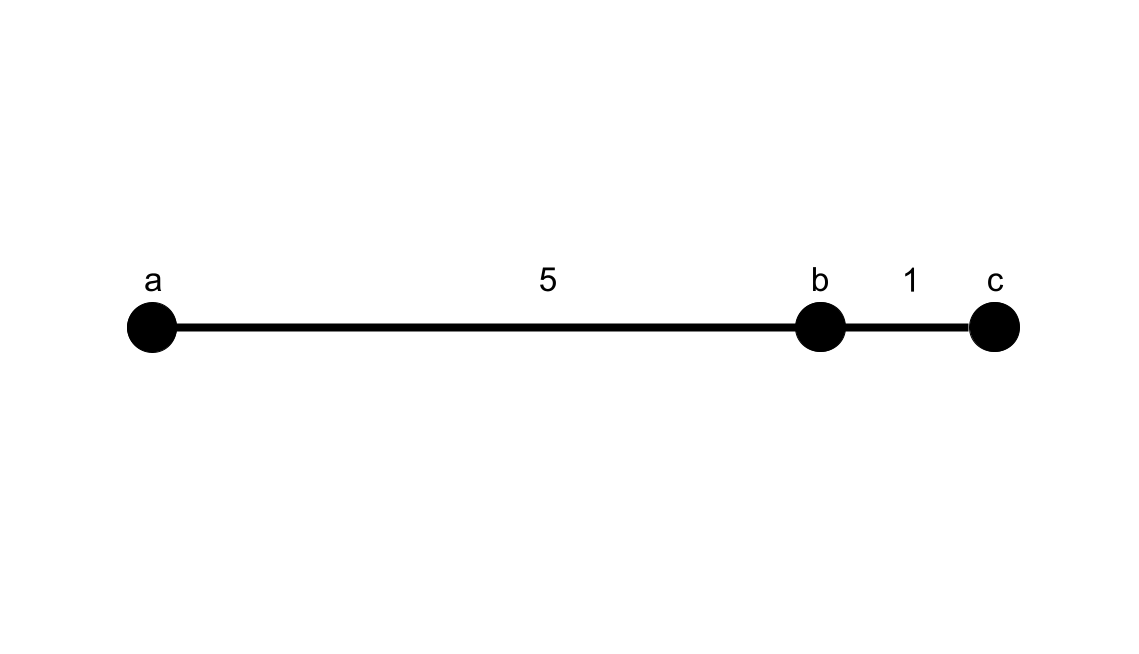
\includegraphics[width=0.5\textwidth]{images/line.png}
        \caption{An example metric space for $GREEDY$'s non-competitiveness}
    \end{figure}
    Suppose we have $k = 2$, and both $GREEDY$ and $OPT$ begin with servers at $b$ and $c$. We begin by requesting $a$, and then proceed to alternate requests between $b$ and $c$. $OPT$ will first service $a$ with the server at $b$, and then move this server back to $b$ incurring a total cost of 10, and from there never increasing. $GREEDY$ will service $a$ with the server at $b$, but then proceed to move the server at $c$ back and forth between $b$ and $c$, in accordance with its policy. Therefore, $GREEDY$ will incur a cost of 1 each time a new request is processed, forever increasing. It is clear that the competitive ratio of $GREEDY$ is unbounded, and therefore $GREEDY$ is not a competitive algorithm.
\end{proof}

\subsubsection*{Bijective Analysis}
While from the worst-case perspective of the competitive ratios $GREEDY$ is worse than $WFA$, Bijective Analysis tells a different story. In this section, we provide some experimental results for the bijective ratios between $WFA$ and $GREEDY$, supporting the results shown in~\cite{bij2016} that $GREEDY$ is actually a bijectively optimal online algorithm.


\begin{table}[!htb]
    \begin{minipage}{.5\linewidth}
      \centering
      \begin{tabular}{|c|c|c|c|c|c|}
        \hline
        Input Number & Space Type & Space Size & Servers & Input Length & Number of Inputs\\
        \hline
        1 & Line & 6 & 2 & 8 & ALL \\
        \hline
        2 & Line & 8 & 2 & 7 & ALL \\
        \hline
        3 & Line & 8 & 3 & 7 & ALL\\
        \hline
        4 & Line & 10 & 3 & 8 & ALL\\
        \hline
        5 & Line & 10 & 3 & 20 & 10,000,000\\
        \hline
        6 & Line & 10 & 3 & 100 & 1,000,000\\
        \hline 
        7 & Circle & 6 & 2 & 8 & ALL\\
        \hline
        8 & Circle & 8 & 3 & 8 & ALL\\
        \hline
        9 & Circle & 10 & 2 & 6 & ALL\\
        \hline
        10 & Circle & 10 & 3 & 6 & ALL\\
        \hline
        11 & Circle & 20 & 3 & 6 & ALL \\
        \hline
    \end{tabular}
        \caption{Tests}
        \label{tab:tests}
    \end{minipage}%
    \\
    \begin{minipage}{.5\linewidth}
        \centering
        \begin{tabular}{|c|c|c|c|}
          \hline
          Input Number & GRE/OPT Bij. & WFA/OPT Bij. & WFA/GRE Bij.\\
          \hline
          1 & 3/2 & 3/2 & 4/3\\
          \hline
          2 & 3/2 & 1.55 & 4/3\\
          \hline
          3 & 3/2 & 1.6 & 4/3 \\
          \hline
          4 & 3/2 & 1.59 & 4/3 \\
          \hline
          5 & 1.319 & 1.308 & 1.03 \\
          \hline
          6 & 1.447 & 1.486 & 1.2 \\
          \hline
          7 & 3/2 & 3/2 & 7/6 \\
          \hline
          8 & 3/2 & 3/2 & 4/3 \\
          \hline
          9 & 3/2 & 3/2 & 7/6 \\
          \hline
          10 & 3/2 & 3/2 & 4/3 \\
          \hline
          11 & 3/2 & 3/2 & 4/3 \\
          \hline

      \end{tabular}
          \caption{Results}
          \label{tab:results}
    \end{minipage} 
\end{table}

The first thing to note is that running these algorithms on a small subset of random inputs of a certain length seems to provide little to no insight into the algorithms true performace. Both $GREEDY$ and $WFA$ perform well - if not optimally - on a large subset of the inputs. As our input lengths increase, the number of possible inputs increases exponentially. To demonstrate the phenomena we observe, suppose for example that $GREEDY$ and $WFA$ perform optimally on 90\% of inputs, and we are able to run 1,000,000,000 inputs of any length on a metric space with 10 points in reasonable time (this is not true, as our computation time increase drastically with regard to input length due to the WFA). So, we can run all inputs of length 9 within this time. If we want to run inputs of length 10, we are only able to run 10\% of the inputs. If we want to run inputs of length 12, we can only run 0.1\% of the inputs! The probability that all of these inputs will land within the 90\% where the algorithms perform optimally increases exponentially as our input length increases, making our bijective ratio approach 1. This is demonstrated in input ID 5 and 6. For both of these we observe smaller experimental bijective ratios than on the inputs where we are able to run all of the possible request sequences. Therefore, we can only start to draw interesting conclusions from the input parameters where we can run every possible input sequence.

The final interesting result is with respect to the comparison between $WFA$ and $GREEDY$. The bijection in the other direction is not shown, as it is always 1 (meaning that $GREEDY$ always performs as well if not better than $WFA$, bijectively). These experimental results support the proofs in~\cite{bij2016} that $GREEDY$ is a bijective optimal algorithm. The fact that the bijective ratio shown is not 1 suggests some interesting results. If both of these bijections could be proven, then this would show that it is better to use $GREEDY$ rather than $WFA$ (a computationally much more expensive algorithm), across a uniform distribution of inputs. For every input where $GREEDY$ performs poorly, there would be an input where $WFA$ performs just as poorly if not worse. This is an interesting result, and suggests that $GREEDY$ is a better algorithm to use in practice.

\subsubsection*{Direct Analysis and Average Case Analysis}
Direct analysis and Average case experiments have been run on the reduced caterpillar graph, and the results are shown in the table below. We provide experiments for a variety of input lengths and metric space sizes, with 2 and 3 servers. For the $WFA$, the direct analysis ratios for all inputs reflect the current belief that it is a $k$ competitive algorithm. It is interesting to note that $GREEDY$ has the same direct analysis ratio for metric spaces of size 12 and 15 for both 2 and 3 servers.

The average case ratios for $GREEDY$ are consistently better than those for $WFA$. This supports the claims made above, that in general for a uniform distribution of inputs, $GREEDY$ is a better algorithm to use in practice. It is worth noting that the current input requests do consider all possible inputs, so a sequence of requests to the same point multiple times in a row is possible. It may be intersting to analyze this problem on a reduced input space, where only a subset of "interesting" inputs are considered.

Unfortunately, average case analysis results were not collected for the 5th input. 

\begin{table}[!htb]
    \begin{minipage}{.5\linewidth}
      \centering
      \begin{tabular}{|c|c|c|c|c|c|}
        \hline
        Input Number & Space Size & Servers & Input Length & Number of Inputs\\
        \hline
        1 & 12 & 2 & 6 & ALL \\
        \hline
        2 & 12 & 3 & 6 & ALL \\
        \hline
        3 & 15 & 2 & 6 & ALL \\
        \hline
        4 & 15 & 3 & 6 & ALL \\
        \hline
        5 & 6 & 3 & 10 & ALL\\
        \hline
        6 & 6 & 3 & 12 & ALL\\
        \hline
        7 & 9 & 3 & 11 & ALL\\
        \hline
    \end{tabular}
        \caption{Tests for Reduced Caterpillar Graphs}
        \label{tab:tests1}
    \end{minipage}%
    \\
    \begin{minipage}{.5\linewidth}
        \centering
        \begin{tabular}{|c|c|c|c|c|}
          \hline
          Input Number & WFA Direct & GREEDY Direct & WFA Avg & GREEDY Avg\\
          \hline
          1 & 2 & 11/3 & 0.783765 & 0.55331442\\
          \hline
          2 & 3 & 3 & 0.845332 & 0.69159289\\
          \hline
          3 & 2 & 11/3 & 0.76000421 & 0.54207148\\
          \hline
          4 & 3 & 3 & 0.870354 & 0.59062018 \\
          \hline
          5 & 3 & 5 &  &  \\
          \hline
          6 & 3 & 6 & 1.50743743999 & 1.236367319548 \\
          \hline
          7 &  &  &  & \\
          \hline

      \end{tabular}
          \caption{Direct Analysis Results}
          \label{tab:results1}
    \end{minipage} 
\end{table}

\section{Conclusion}
\label{sec:con}
In this work, we analyze the \KS problem and provide descriptions for various algorithms. We primarily focus on the most common form of analysis for the \KS problem (competitive analysis). We provide an overview of various theorems and proofs taken from~\cite{OnlineComp1998}, and additionally go over a fast min-cut max-flow formulation for computing the $\mathrm{WFA}$ movement~\cite{mcfp2011}. We then transition to focusing on the Unifying Potential~\cite{unifyingPotential2021}, overviewing a few of their definitions and proofs. We attempt to extend their methods for multiray spaces to reduced caterpillar graphs. We consider the symetry property they demonstrate for their modified potential, and attempt to extend this to our reduced caterpillar graphs. Finally, we describe various other analysis methods used in the context of this problem, including bijective analysis, the Max-Max ratio, and a modified average case analysis. We provide an open-source software framework for testing and comparing these algorithms in various environments, as well as a framework for generating metric spaces and input sequences. The software package can be found here: \url{https://github.com/StefanCaldararu/KServers}. We finally provide some experimental results derived using this software, and a brief description of these results.

Potential future extensions of this work would primarily include a completion of the extension of the unifying potential to the reduced caterpilar graphs. This may lead to a potential extension to general tree graphs, and potentially to general metric spaces. Additionally, we could extend the experimental analysis to a wider variety of metric spaces. With more time alloted to computation, we could additionally run experiments on longer request sequences, which may offer further valuable insights.


\bibliographystyle{ieeetr}
\bibliography{refs.bib}


\end{document}          